% Rapport de mini-projet : architecture Zero Trust sur Kubernetes
% Compilation : xelatex rapport.tex (deux fois, pour la table des matieres)
\documentclass[11pt,a4paper]{article}

\usepackage{fontspec}
\usepackage{polyglossia}
\setdefaultlanguage{french}
\usepackage[a4paper,top=2.3cm,bottom=2.3cm,left=2.3cm,right=2.3cm,headheight=14pt]{geometry}
\usepackage{microtype}
\usepackage{graphicx}
\usepackage{booktabs}
\usepackage{tabularx}
\usepackage{array}
\usepackage{float}
\usepackage[font=small,labelfont=bf,labelsep=period]{caption}
\usepackage{listings}
\usepackage{xcolor}
\usepackage{fancyhdr}
\usepackage{titlesec}
\usepackage[hidelinks]{hyperref}
\usepackage{enumitem}

% ---------- champs a completer ----------
\newcommand{\encadrant}{Pr.~Mohammed \textsc{Airaj}}
\newcommand{\video}{\url{https://drive.google.com/file/d/1gj5EWyhtxk6pGZi1-1RBWAKOx2ShKWZ_/view?usp=drive_link}}
% ----------------------------------------

\setlength{\parindent}{0pt}
\setlength{\emergencystretch}{3em}
\setlength{\parskip}{0.55em}
\linespread{1.05}
\setlist{itemsep=0.15em,topsep=0.3em}

\titleformat{\section}{\large\bfseries}{\thesection.}{0.6em}{}
\titleformat{\subsection}{\normalsize\bfseries}{\thesubsection.}{0.6em}{}
\titlespacing*{\section}{0pt}{1.2em}{0.5em}
\titlespacing*{\subsection}{0pt}{0.9em}{0.3em}

\pagestyle{fancy}
\fancyhf{}
\fancyhead[L]{\small\textit{Architecture Zero Trust sur Kubernetes}}
\fancyhead[R]{\small\textit{ENSA Fès, GDNC}}
\fancyfoot[C]{\small\thepage}
\renewcommand{\headrulewidth}{0.4pt}

\lstset{basicstyle=\ttfamily\footnotesize,columns=fullflexible,frame=single,
  framerule=0.3pt,rulecolor=\color{gray!60},xleftmargin=2pt,xrightmargin=2pt,
  aboveskip=0.6em,belowskip=0.4em,breaklines=true}

\newcolumntype{L}{>{\raggedright\arraybackslash}X}
\newcommand{\code}[1]{\texttt{#1}}

\begin{document}

% ======================= PAGE DE GARDE =======================
\begin{titlepage}
\centering
{\large Université Sidi Mohamed Ben Abdellah\par}
\vspace{0.2cm}
{\large\bfseries École Nationale des Sciences Appliquées de Fès\par}
\vspace{0.2cm}
{Filière Génie du Développement Numérique et Cybersécurité (GDNC)\par}
\vspace{2.8cm}
{\large Rapport de mini-projet, module DevSecOps\par}
\vspace{0.8cm}
\rule{\textwidth}{0.6pt}\par
\vspace{0.4cm}
{\LARGE\bfseries Sécurisation des workloads Kubernetes\\[0.25cm] selon une approche Zero Trust\par}
\vspace{0.4cm}
\rule{\textwidth}{0.6pt}\par
\vspace{0.6cm}
{\large Conception, mise en œuvre et mesure des résultats\par}
\vspace{3cm}
\begin{minipage}[t]{0.47\textwidth}
\raggedright
\textit{Réalisé par :}\\[0.2cm]
Abir \textsc{Majdi}\\
Doha \textsc{El Merabet}
\end{minipage}\hfill
\begin{minipage}[t]{0.47\textwidth}
\raggedleft
\textit{Encadré par :}\\[0.2cm]
\encadrant
\end{minipage}
\vfill
{Année universitaire 2026--2027\par}
\vspace{0.2cm}
{\small Remis le 9 novembre 2026\par}
\end{titlepage}

% ======================= TABLE DES MATIERES =======================
\pagenumbering{roman}
\tableofcontents
\newpage
\pagenumbering{arabic}

% ======================= INTRODUCTION =======================
\section{Introduction}

Les clusters Kubernetes partagés entre plusieurs applications posent un problème de confiance implicite. Par défaut, tout pod peut joindre tout autre pod, chaque compte de service reçoit un jeton monté automatiquement, et le serveur d'API accepte des conteneurs privilégiés tant qu'aucune règle d'admission ne s'y oppose. Une seule application compromise suffit alors à atteindre le reste du cluster.

Le modèle Zero Trust, formalisé par le NIST \cite{nist207}, part du principe inverse : aucune communication ni aucun accès n'est accordé sur la seule base de la position dans le réseau, et chaque autorisation doit être explicite. Le sujet de ce mini-projet pose la question suivante :

\begin{quote}
\itshape Comment appliquer le principe Zero Trust aux workloads Kubernetes sans multiplier inutilement les mécanismes de sécurité ?
\end{quote}

Nous avons choisi d'y répondre par la mesure. L'application est d'abord déployée sans aucune protection, puis quatre scénarios d'attaque sont rejoués (tableau~\ref{tab:scenarios}). Les couches de sécurité sont ensuite ajoutées une par une, et les mêmes scénarios sont rejoués après chacune. Un outil n'est conservé que s'il réduit un risque mesuré que les couches précédentes ne couvraient pas déjà.

\begin{table}[H]
\centering
\caption{Scénarios d'attaque rejoués après chaque couche. Dans tous les cas, l'attaquant exécute du code dans le pod frontend.}
\label{tab:scenarios}
\begin{tabularx}{\textwidth}{@{}l L l@{}}
\toprule
\textbf{ID} & \textbf{Scénario} & \textbf{MITRE ATT\&CK} \\
\midrule
S1 & Mouvement latéral depuis le frontend compromis & T1046, T1059 \\
S2 & Vol du jeton du compte de service & T1528, T1552.007 \\
S3 & Déploiement d'un pod privilégié avec \code{hostPath} & T1610, T1611 \\
S4 & Fuite du mot de passe de la base de données & T1552 \\
\bottomrule
\end{tabularx}
\end{table}

Le travail a été réparti en deux parties. Abir \textsc{Majdi} (partie~A) a traité les identités et le RBAC, le réseau avec Cilium, l'admission avec Pod Security Admission et Kyverno, ainsi que l'intégration continue. Doha \textsc{El Merabet} (partie~B) a traité la gestion des secrets avec Vault et External Secrets Operator, l'audit de l'API, le chiffrement au repos, la détection avec Falco, l'analyse des images avec Trivy et les schémas d'architecture. Chacune a relu et testé le travail de l'autre. Tout le code et les preuves sont publiés dans le dépôt du projet \cite{depot}.

% ======================= ARCHITECTURE =======================
\section{Architecture et environnement de test}

\subsection{Application et composants}

L'application de démonstration comporte trois tiers, chacun isolé dans son propre namespace : un frontend \code{nginx-unprivileged}, une API \code{podinfo} et une base PostgreSQL disposant d'un volume persistant de 1~Gi. Un quatrième namespace, \code{zt-attacker}, héberge un pod qui simule un attaquant interne. Les outils de sécurité sont installés chacun dans un namespace dédié (tableau~\ref{tab:composants}).

\begin{table}[H]
\centering
\caption{Composants déployés et versions figées dans \code{versions.md}.}
\label{tab:composants}
\begin{tabularx}{\textwidth}{@{}l L@{}}
\toprule
\textbf{Namespace} & \textbf{Composant} \\
\midrule
\code{zt-frontend}, \code{zt-api}, \code{zt-data} & Frontend (port 8080), API (port 9898), PostgreSQL 16 (port 5432) \\
\code{zt-attacker} & Pod attaquant, image \code{curl:8.10.1} \\
\code{kube-system} & Cilium 1.20.4 et Hubble, CoreDNS \\
\code{kyverno} & Kyverno 1.19.2 \\
\code{vault}, \code{external-secrets} & Vault 2.0.4 (stockage Raft), External Secrets Operator 2.14.0 \\
\code{falco} & Falco 0.45.2, Falcosidekick et son interface \\
\bottomrule
\end{tabularx}
\end{table}

Les deux membres du binôme disposent chacun d'un cluster k3s v1.36.5 à un seul nœud : \code{zt-lab-a} sous Debian~13 et \code{zt-lab-b} sous Ubuntu~24.04. k3s est installé sans Flannel, sans Traefik et sans son contrôleur de NetworkPolicy intégré, de sorte que Cilium soit à la fois le seul CNI et le seul moteur de politiques réseau. Disposer de deux systèmes différents nous a permis de vérifier que les résultats ne dépendent pas d'une machine particulière.

\subsection{Frontières de confiance}

Nous avons identifié cinq frontières. Internet n'entre dans l'application que par le frontend. Chaque tier ne communique qu'avec le suivant : le frontend avec l'API sur le port 9898, l'API avec la base sur le port 5432. Les pods applicatifs n'ont aucun besoin de l'API Kubernetes et ne reçoivent donc aucun jeton. Seul le contrôleur d'External Secrets Operator dialogue avec Vault. Enfin, seuls Cilium et Falco franchissent la frontière avec le noyau du nœud, par eBPF, ce qui en fait des composants privilégiés à protéger. La figure~\ref{fig:archi} montre ce qu'il reste à un attaquant installé dans le frontend une fois toutes les couches en place.

\begin{figure}[H]
\centering
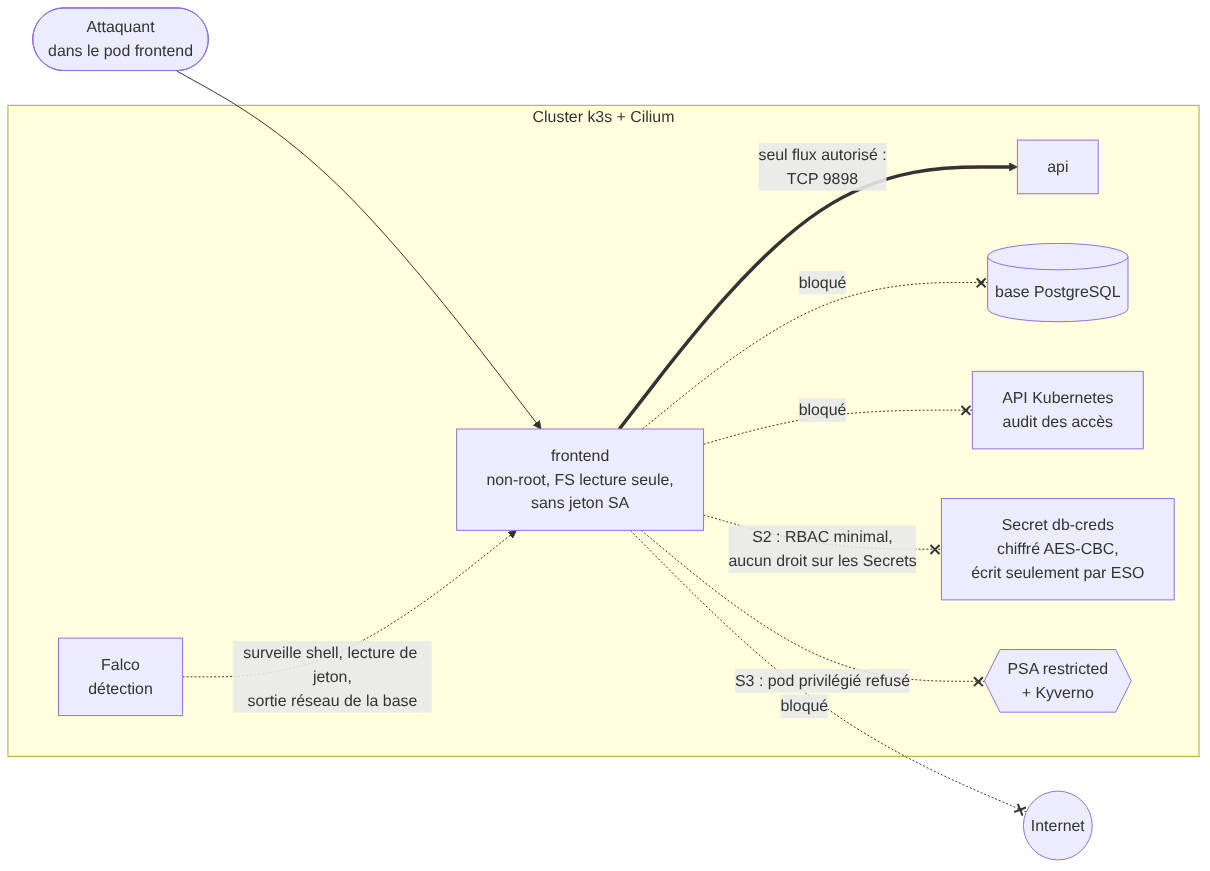
\includegraphics[width=0.85\textwidth]{img/architecture-apres.png}
\caption{Surface accessible depuis le pod frontend compromis après mise en place de toutes les couches (schéma issu de \code{docs/architecture/README.md}).}
\label{fig:archi}
\end{figure}

\subsection{Démarche et organisation du travail}

Le projet a été conduit par phases, chacune ajoutant une couche de sécurité puis rejouant les quatre scénarios (tableau~\ref{tab:phases}). Les tâches étaient suivies dans un tableau GitHub Projects, à raison d'un ticket par tâche, attribué à son autrice et fermé uniquement lorsque la preuve correspondante était enregistrée dans \code{docs/evidence/}. Les commits sont signés par clé SSH et un crochet Gitleaks empêche l'envoi de tout secret dans le dépôt.

\begin{table}[H]
\centering
\caption{Phases du projet et répartition du travail.}
\label{tab:phases}
\small
\begin{tabularx}{\textwidth}{@{}l L l l@{}}
\toprule
\textbf{Phase} & \textbf{Contenu} & \textbf{Responsable} & \textbf{Cluster} \\
\midrule
0 & Dépôt, modèle de menaces, contrat d'interface (noms, ports, labels) & A. Majdi & \\
1 & Installation de k3s et Cilium, application sans protection, mesure de référence & les deux & a et b \\
2 à 4 & RBAC, NetworkPolicy et Cilium, Pod Security Admission, Kyverno & A. Majdi & a \\
5 & Vault et External Secrets Operator & D. El Merabet & b \\
6 & Audit de l'API, chiffrement au repos, Falco & D. El Merabet & b \\
7 & Intégration de toutes les couches et nouvelle mesure de S1 à S4 & les deux & a et b \\
8 et 9 & Conformité, relecture croisée, reconstruction depuis zéro, rapport & les deux & a et b \\
\bottomrule
\end{tabularx}
\end{table}

% ======================= PARTIE A =======================
\section{Partie A : identités, réseau et admission}

\subsection{Comptes de service et RBAC}

Dans la configuration initiale, le compte \code{sa-frontend} disposait du rôle \code{edit} dans les trois namespaces applicatifs, soit 96 règles dans \code{zt-data}. Or aucun composant de l'application n'interroge l'API Kubernetes. Le moindre privilège revient donc ici à n'accorder aucune permission : les cinq comptes de service applicatifs n'ont aucun Role, et l'option \code{automount\-Service\-Account\-Token:~false} est positionnée sur chaque compte et sur chaque pod.

Après cette étape, \code{sa-frontend} ne conserve que les 23 règles de découverte accordées par défaut à tout compte authentifié. Nous avons vérifié avec \code{kubectl auth can-i} que les cinq comptes ne peuvent ni lire les Secrets, ni créer de pods, ni utiliser \code{pods/exec}, ni créer de RoleBinding, ni recourir aux verbes \code{escalate}, \code{bind} ou \code{impersonate}. Les scénarios S2 et S4 sont ainsi fermés au niveau de l'API.

\subsection{Segmentation réseau avec Cilium}

Chaque namespace applicatif reçoit une politique de refus par défaut, en entrée comme en sortie, puis une règle autorisant le DNS et une politique par flux légitime. Avant de nous appuyer sur ces règles, nous avons vérifié que le CNI les applique réellement : sans politique, une requête de l'attaquant vers l'API aboutit, alors qu'avec une politique de refus en sortie elle expire (figure~\ref{fig:netpol}).

\begin{figure}[H]
\centering
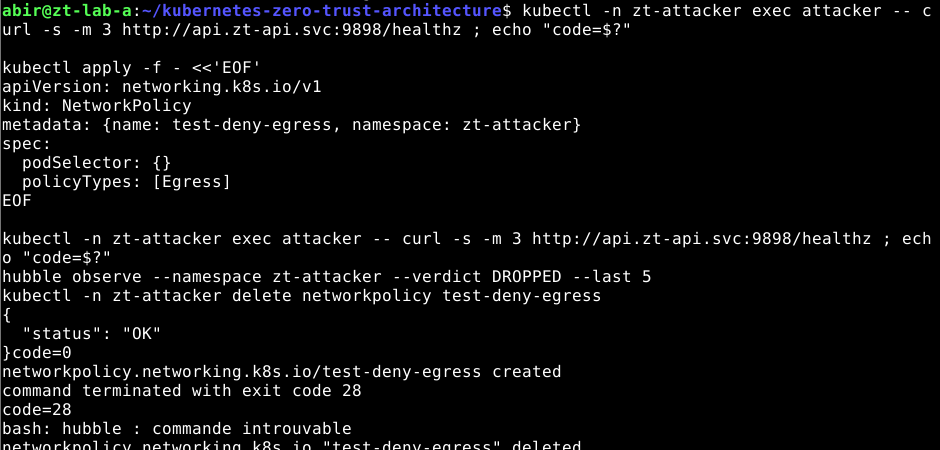
\includegraphics[width=0.62\textwidth]{img/test-networkpolicy.png}
\caption{Vérification de l'application des NetworkPolicy : la même requête renvoie \code{code=0}, puis \code{code=28} (délai dépassé) après création de la politique.}
\label{fig:netpol}
\end{figure}

Hubble, l'outil d'observation de Cilium, confirme le résultat du côté du frontend. L'extrait suivant, abrégé, provient de la capture du 7 novembre 2026 conservée dans le dépôt :

\begin{lstlisting}
zt-frontend/frontend -> zt-data/database:5432   Policy denied DROPPED (TCP Flags: SYN)
zt-frontend/frontend -> 10.0.2.15:6443 (host)   Policy denied DROPPED (TCP Flags: SYN)
zt-frontend/frontend -> 1.1.1.1:443 (world)     Policy denied DROPPED (TCP Flags: SYN)
\end{lstlisting}

Le frontend ne joint donc plus ni la base, ni l'API Kubernetes, ni Internet. Le tableau~\ref{tab:flux} récapitule les flux autorisés et les flux refusés que nous avons testés.

\begin{table}[H]
\centering
\caption{Matrice des flux réseau après la phase de segmentation.}
\label{tab:flux}
\small
\begin{tabularx}{\textwidth}{@{}L l l@{}}
\toprule
\textbf{Flux} & \textbf{Résultat} & \textbf{Règle} \\
\midrule
frontend vers API, TCP 9898 & autorisé & \code{allow-frontend-to-api} \\
API vers base, TCP 5432 & autorisé & \code{allow-api-to-database} \\
pods applicatifs vers CoreDNS, port 53 & autorisé & \code{allow-dns-egress} \\
ESO vers Vault, TCP 8200 & autorisé & \code{network/40-vault-eso.yaml} \\
Falco vers Falcosidekick & autorisé & \code{network/50-falco.yaml} \\
frontend vers base, API Kubernetes ou Internet & refusé & refus par défaut \\
pod attaquant vers Vault, TCP 8200 & refusé & refus par défaut \\
\bottomrule
\end{tabularx}
\end{table}

 Une politique CiliumNetworkPolicy de niveau~7 a également été testée (\code{GET /healthz} autorisé, \code{GET /version} refusé). Nous l'avons gardée comme démonstration plutôt que de l'étendre à tous les flux, afin de ne pas rendre chaque manifeste dépendant de Cilium.

\subsection{Contrôle d'admission}

Tous les namespaces applicatifs appliquent le profil \code{restricted} de Pod Security Admission \cite{k8s}, qui rejette le pod privilégié de S3 avant même l'intervention de Kyverno. Kyverno ne sert donc qu'à exprimer ce que PSA ne sait pas exprimer (tableau~\ref{tab:kyverno}).

\begin{table}[H]
\centering
\caption{Politiques Kyverno appliquées aux namespaces \code{zt-*}.}
\label{tab:kyverno}
\footnotesize
\begin{tabularx}{\textwidth}{@{}l l L@{}}
\toprule
\textbf{Politique} & \textbf{Type} & \textbf{Effet} \\
\midrule
\code{best-practices-disallow-latest-tag} & validation & Refuse les images sans tag ou marquées \code{latest} \\
\code{best-practices-require-limits} & validation & Impose des limites CPU et mémoire \\
\code{supply-chain-restrict-images} & validation & N'admet que les images d'une liste blanche \\
\code{defaults-mutate-pod-defaults} & mutation & Ajoute des paramètres de sécurité par défaut \\
\code{defaults-generate-default-deny} & génération & Crée un refus par défaut dans chaque nouveau namespace \\
\code{secrets-only-from-eso} & validation & Réserve l'écriture des Secrets de \code{zt-data} à ESO \\
\bottomrule
\end{tabularx}
\end{table}

La relecture croisée par Doha \textsc{El Merabet} a mis au jour deux failles réelles dans ces politiques. La première (R1) permettait de contourner les règles de tag, de limites et de liste blanche en plaçant l'image dans un \code{initContainer}. La seconde (R10) tenait au fait que Kyverno tolère par défaut les violations existantes : un Secret déjà présent dans \code{zt-data} restait modifiable par l'administrateur. L'option \code{allowExistingViolations: false} \cite{kyverno} a corrigé ce point. Les deux corrections ont été retestées sur les deux clusters.

Nous avons aussi mesuré le comportement de Kyverno en cas de panne. Avec un seul réplica, un arrêt propre retire les webhooks et le cluster admet alors tout pod (\textit{fail-open}), tandis qu'un arrêt brutal laisse les webhooks en place et bloque toute création de pod pendant une trentaine de secondes (\textit{fail-closed}). Trois réplicas protégés par un PodDisruptionBudget constitueraient la parade habituelle, que notre machine à un seul nœud ne permettait pas de tester.

Deux choix méritent d'être signalés. Une exception documentée (\code{PolicyException}) autorise le tag \code{latest} pour les seuls pods de test nommés \code{latest-exception-*} dans \code{zt-attacker}, ce qui montre comment déroger à une règle sans la désactiver. Par ailleurs, les politiques sont passées directement en mode \code{Enforce}, car le laboratoire ne contenait aucune charge existante. En production, il faudrait d'abord les appliquer en mode \code{Audit} et examiner les rapports, afin de ne pas bloquer les applications déjà en place.

\begin{figure}[H]
\centering
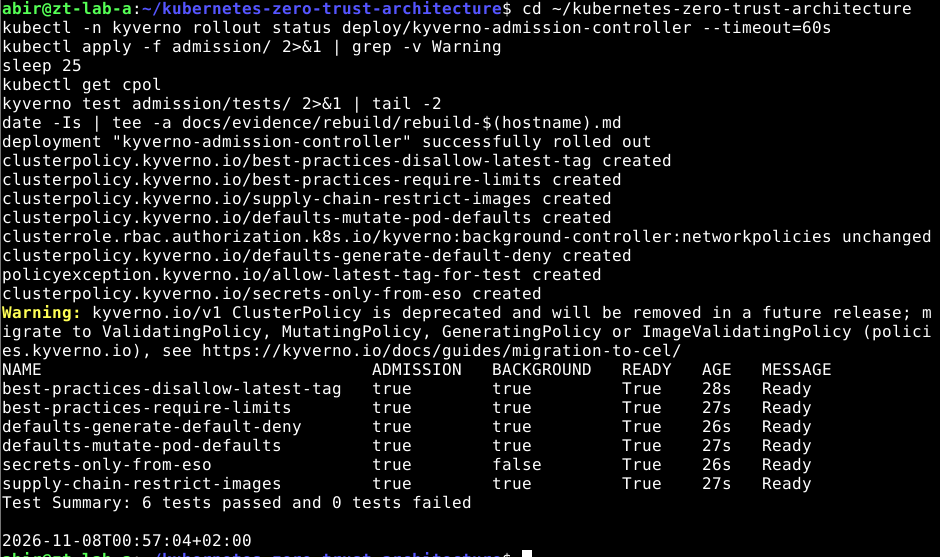
\includegraphics[width=0.6\textwidth]{img/kyverno-tests.png}
\caption{Politiques Kyverno prêtes et six tests \code{kyverno test} réussis lors de la reconstruction de \code{zt-lab-a}.}
\label{fig:kyverno}
\end{figure}

\subsection{Mesure automatisée et reproductibilité}

Le script \code{scripts/measure.sh} rejoue les quatre scénarios depuis le pod frontend et enregistre le résultat dans \code{docs/evidence/} (figure~\ref{fig:mesure}). Une chaîne d'intégration continue GitHub Actions exécute Gitleaks sur tout l'historique et les tests Kyverno à chaque envoi. Le 8 novembre 2026, \code{zt-lab-a} a été entièrement détruit puis reconstruit en suivant uniquement le README, en 47 minutes. Les six critères d'acceptation ont été satisfaits et la mesure obtenue est identique à celle du cluster d'origine.

\begin{figure}[H]
\centering
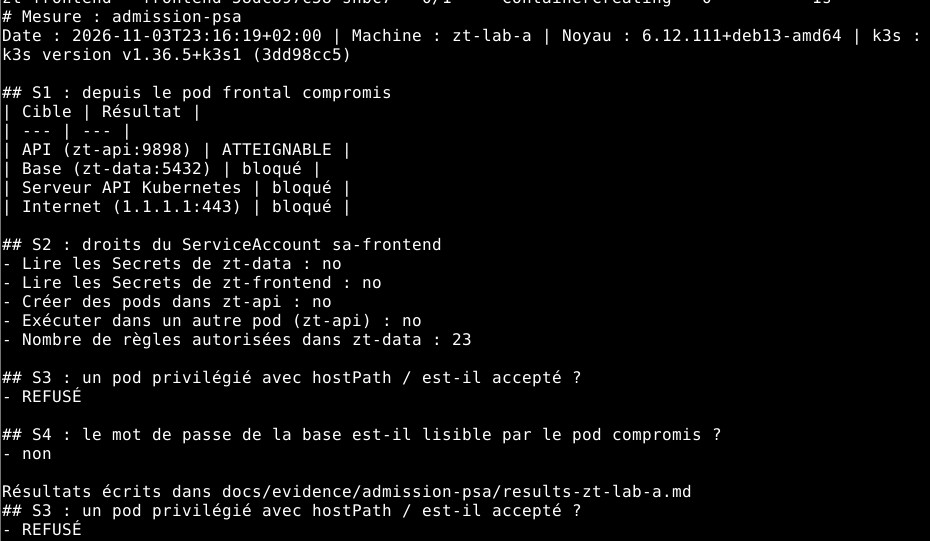
\includegraphics[width=0.55\textwidth]{img/mesure-s1-s4.png}
\caption{Sortie de \code{measure.sh} après l'ajout de PSA : seule l'API reste atteignable et les scénarios S2 à S4 échouent.}
\label{fig:mesure}
\end{figure}

% ======================= PARTIE B =======================
\section{Partie B : secrets, traçabilité et détection}

\subsection{Gestion des secrets avec Vault et External Secrets Operator}

Dans la configuration initiale, le mot de passe de la base est un Secret Kubernetes créé à la main. Il n'est qu'encodé en base64, n'a pas d'historique et n'est jamais renouvelé. Vault devient la source de vérité unique : External Secrets Operator (ESO) recopie la valeur dans le Secret \code{db-creds}, que PostgreSQL lit sans modification.

Vault fonctionne avec un stockage Raft persistant, hors mode développement, et le moteur KV~v2 conserve les versions successives du secret. Le rôle d'authentification \code{eso} n'accepte que le compte \code{eso-vault} du namespace \code{zt-data}, avec l'audience \code{vault} et un jeton valable 15 minutes, et la politique associée ne permet de lire que le chemin \code{secret/data/zt/database/*}. Nous avons préféré ESO au sidecar Vault Agent pour deux raisons : l'application n'a pas à être modifiée, et aucun pod applicatif n'a besoin de communiquer avec Vault. Le tableau~\ref{tab:secrets} compare les trois approches envisagées.

\begin{table}[H]
\centering
\caption{Comparaison des approches de gestion des secrets.}
\label{tab:secrets}
\small
\begin{tabularx}{\textwidth}{@{}l L L L@{}}
\toprule
\textbf{Critère} & \textbf{Secret natif} & \textbf{Vault et sidecar Agent} & \textbf{Vault et ESO (retenu)} \\
\midrule
Source de vérité & datastore du cluster & Vault & Vault \\
Modification de l'application & aucune & annotations, lecture de fichiers & aucune \\
Flux réseau des pods vers Vault & sans objet & oui, depuis chaque pod & non, seul le contrôleur ESO \\
Rotation et historique & manuels, aucun & oui & oui (versions KV) \\
Composants ajoutés & aucun & webhook d'injection et un sidecar par pod & un opérateur \\
Risque principal & toute identité ayant \code{get secrets} & webhook d'injection, nombreux clients Vault & ESO peut lire et écrire les Secrets de \code{zt-data} \\
\bottomrule
\end{tabularx}
\end{table}



Les tests confirment le cloisonnement. Une connexion au rôle \code{eso} avec un jeton volé de \code{sa-frontend} ou de \code{sa-attacker} est refusée, aucun compte applicatif ne peut lire \code{db-creds}, et le mot de passe n'apparaît nulle part dans le dépôt Git. Le script de rotation change le mot de passe dans PostgreSQL, écrit une nouvelle version dans Vault, force la synchronisation puis vérifie une connexion réelle à la base (figure~\ref{fig:vault}). Lorsque Vault redémarre scellé, ESO passe en erreur de synchronisation mais l'application continue de fonctionner avec la dernière valeur connue.

\begin{figure}[H]
\centering
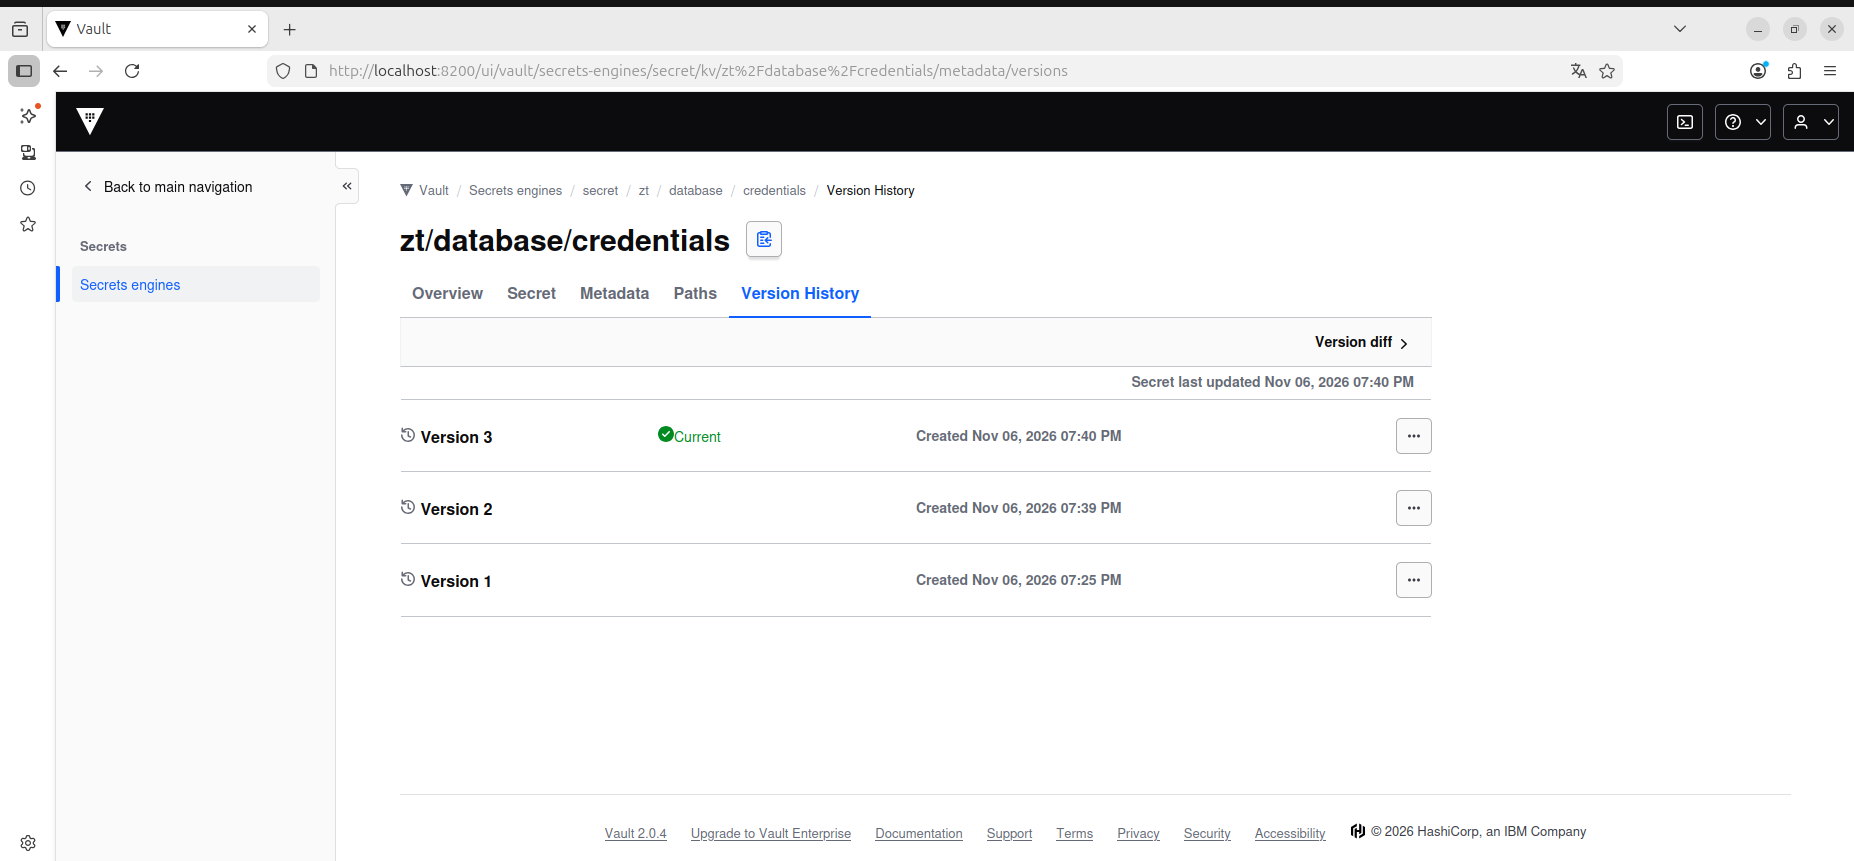
\includegraphics[width=0.7\textwidth]{img/vault-versions.png}
\caption{Historique du secret de la base dans Vault : la copie initiale et deux rotations.}
\label{fig:vault}
\end{figure}

\subsection{Audit de l'API et chiffrement au repos}

La politique d'audit enregistre les accès aux Secrets au niveau \code{Metadata}, c'est-à-dire l'auteur, l'action et la date sans jamais le contenu, et conserve le corps complet des modifications sensibles (RBAC, NetworkPolicy, politiques Kyverno). Le journal fait apparaître l'exécution d'une commande dans le frontend ainsi que la tentative de lecture de \code{db-creds} par l'identité volée, refusée avec le code 403. La valeur du mot de passe n'y figure jamais.

Le chiffrement au repos des Secrets proposé par k3s (AES-CBC) a été activé, puis tous les Secrets existants ont été rechiffrés. Un marqueur de test, lisible en clair dans la base de données du nœud avant l'activation, ne l'est plus ensuite : la valeur stockée commence désormais par \code{k8s:enc:aescbc:v1:}.

\subsection{Détection à l'exécution avec Falco}

Falco, avec le pilote \code{modern\_ebpf}, porte cinq règles propres au projet, chacune rattachée à un scénario et à une technique MITRE ATT\&CK (tableau~\ref{tab:falco}).

\begin{table}[H]
\centering
\caption{Règles Falco écrites pour le projet.}
\label{tab:falco}
\small
\begin{tabularx}{\textwidth}{@{}L l l l@{}}
\toprule
\textbf{Règle} & \textbf{Scénario} & \textbf{ATT\&CK} & \textbf{Priorité} \\
\midrule
Shell lancé dans un conteneur applicatif & S1 & T1059 & Warning \\
Lecture du jeton de compte de service & S2 & T1528 & Warning \\
Connexion sortante depuis le tier de données & S1, S4 & T1041 & Notice \\
Accès interactif aux outils de secrets & S4 & T1552 & Critical \\
Lecture du stockage de Vault par un autre processus & S4 & T1552.001 & Critical \\
\bottomrule
\end{tabularx}
\end{table}

La règle de connexion sortante signale également les tentatives que les NetworkPolicy bloquent, si bien qu'une même attaque est à la fois empêchée par Cilium et détectée par Falco (figure~\ref{fig:falco}). Un faux positif, causé par la sonde de disponibilité de Vault et déclenché toutes les cinq secondes, a été supprimé par une exception documentée.

\begin{figure}[H]
\centering
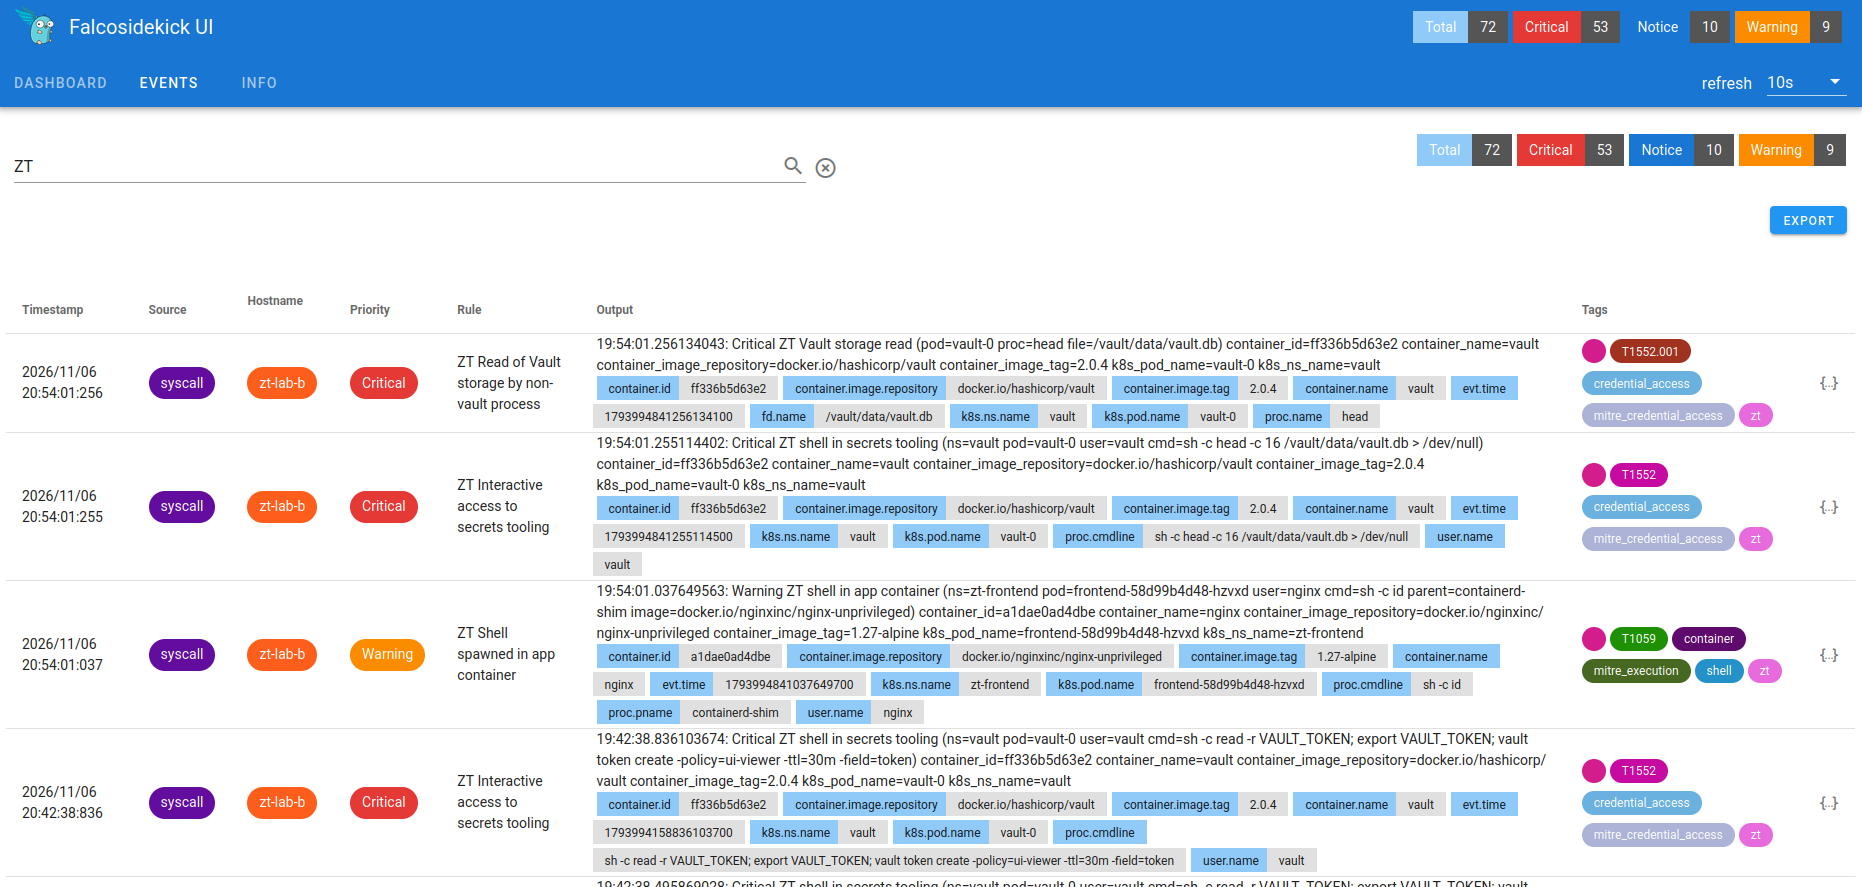
\includegraphics[width=0.85\textwidth]{img/falco-events.png}
\caption{Alertes du projet dans Falcosidekick, avec leur priorité, le pod concerné et l'étiquette MITRE.}
\label{fig:falco}
\end{figure}

\subsection{Analyse des images et seconde reconstruction}

Trivy recense 222 vulnérabilités de niveau élevé ou critique dans les quatre images applicatives : 65 pour nginx-unprivileged, 107 pour podinfo, 26 pour postgres et 24 pour curl. Toutes disposent d'une version corrigée et aucune ne provient de la configuration du cluster. Pour nginx-unprivileged, podinfo et curl, la cause est un système de base Alpine ancien, auquel s'ajoutent pour podinfo deux binaires Go compilés avec une version ancienne de Go. Pour postgres, au contraire, le système Alpine~3.24 est récent et sans faille de ce niveau : les 26 résultats viennent tous du binaire Go \code{gosu} embarqué dans l'image. Nous les avons acceptées dans le cadre du laboratoire, car changer de versions juste avant la remise aurait invalidé les mesures ainsi que la liste blanche de Kyverno. En production, il faudrait mettre à jour les images, les référencer par leur empreinte et ajouter Trivy à la chaîne d'intégration continue pour bloquer toute image présentant une faille critique corrigeable.

Le 8 novembre 2026, \code{zt-lab-b} a lui aussi été reconstruit à partir du README, en 55 minutes. Les six critères ont été satisfaits et la mesure obtenue est identique à celle de \code{zt-lab-a}. Cette seconde reconstruction, menée sur un autre système et par l'autre membre du binôme, a révélé d'autres manques que la première : la liste des outils à installer au préalable, le répertoire \code{/etc/cni/net.d} laissé en place par la désinstallation de k3s, l'attente de l'enregistrement du nœud avant les vérifications, et un délai d'attente trop court dans le script de descellement de Vault. Tous ont été corrigés depuis.

% ======================= RESULTATS =======================
\section{Résultats et évaluation}

\subsection{Réduction du rayon d'action}

Le tableau~\ref{tab:blast} résume ce que peut faire le pod frontend compromis à chaque étape. Le RBAC ferme l'accès aux Secrets et la création de pods, les NetworkPolicy coupent les trois cibles réseau illégitimes, et PSA rejette le pod dangereux. Vault, ESO et Falco ne modifient pas ces colonnes, car ils agissent sur d'autres risques : qui peut obtenir le secret, son renouvellement, et la visibilité de l'attaque. La même mesure, rejouée sur \code{zt-lab-b}, donne un résultat identique ligne par ligne.

\begin{table}[H]
\centering
\caption{Rayon d'action du frontend compromis après chaque couche (source : \code{docs/evidence/blast-radius.md}).}
\label{tab:blast}
\small
\begin{tabular}{@{}lcccccccc@{}}
\toprule
\textbf{Étape} & \textbf{API} & \textbf{Base} & \textbf{API K8s} & \textbf{Internet} & \textbf{Secrets} & \textbf{Pods} & \textbf{S3} & \textbf{S4} \\
\midrule
Initiale       & oui & oui & oui & oui & oui & oui & accepté & lisible \\
+ RBAC         & oui & oui & oui & oui & non & non & accepté & non \\
+ NetworkPolicy& oui & non & non & non & non & non & accepté & non \\
+ PSA          & oui & non & non & non & non & non & refusé & non \\
+ Kyverno      & oui & non & non & non & non & non & refusé & non \\
Intégration    & oui & non & non & non & non & non & refusé & non \\
\bottomrule
\end{tabular}
\end{table}

\subsection{Conformité et coût}

Le banc d'essai kube-bench (référentiel CIS \code{k3s-cis-1.9}) donne 59 contrôles réussis et 4 en échec après deux corrections. Les quatre échecs restants ont été analysés : deux faux positifs liés au chemin du CNI, un contrôle non applicable puisque k3s utilise SQLite et non etcd, et un écart justifié, les composants système ayant besoin de leur jeton. Sur \code{zt-lab-b}, le résultat passe de 57 réussis et 6 échecs à 59 réussis et 4 échecs. Kubescape (référentiels NSA et MITRE) a relevé un seul défaut sur nos workloads, le contrôle C-0013 lié à un \code{runAsGroup} manquant, qui a été corrigé. Les 46 ressources encore signalées appartiennent toutes à des composants tiers ou à k3s.

Ce niveau de protection a un coût. Mesurée au repos sur \code{zt-lab-b} avec \code{kubectl top}, l'application occupe 35~MiB de mémoire, alors que Kyverno en occupe 306, Cilium et Hubble 303, ESO 124, Falco et ses composants 116, et Vault 46. Les outils de sécurité consomment donc environ 26 fois plus de mémoire que l'application qu'ils protègent. Sur un cluster de production, ce coût serait partagé entre de nombreuses applications, mais il confirme que chaque outil doit justifier sa présence.

\subsection{Sécurité du stockage}

La base PostgreSQL utilise un volume persistant de 1~Gi fourni par le provisionneur \code{local-path} de k3s, qui crée un répertoire sur le nœud. Le pod tourne sans droits root, le groupe \code{postgres} (\code{fsGroup: 70}) possède le volume, et aucun autre pod ne le monte. Dans chaque pod applicatif, le système de fichiers racine est en lecture seule : seuls des volumes \code{emptyDir}, qui disparaissent avec le pod, sont accessibles en écriture. Les Secrets sont chiffrés au repos et les données de Vault sont protégées par sa propre clé de chiffrement.

Le volume \code{hostPath} est la configuration la plus dangereuse, car il monte un répertoire du nœud dans le conteneur. Avec \code{hostPath: /}, comme dans le scénario S3, un conteneur peut lire \code{/etc/shadow} et les identifiants de k3s, y compris la clé de chiffrement des Secrets, puis prendre le contrôle du nœud. Le profil \code{restricted} de PSA n'autorise que des types de volumes sûrs (\code{configMap}, \code{emptyDir}, \code{persistentVolumeClaim}, \code{projected}, \code{secret}, entre autres) et rejette donc ce pod.

\subsection{Limites}
\label{sec:limites}

La principale limite tient au nœud unique : un attaquant qui compromet le nœud contourne l'ensemble des contrôles. Le flux légitime du frontend vers l'API reste par ailleurs ouvert et pourrait être détourné. Plusieurs raccourcis propres au laboratoire subsistent : Vault fonctionne sans TLS et avec une seule clé de descellement, la clé de chiffrement au repos et les journaux d'audit résident sur le même nœud, et Kyverno ne compte qu'un réplica. Les images applicatives ne sont ni à jour ni référencées par leur empreinte. Le DNS reste un canal d'exfiltration possible et le trafic entre pods n'est pas chiffré. Enfin, Falco détecte sans bloquer, et un Falco arrêté constituerait un angle mort silencieux.

% ======================= QUESTIONS =======================
\section{Réponses aux questions d'analyse du sujet}

\textbf{Quels sont les composants les plus sensibles ?} Par ordre d'importance : le serveur d'API et sa base de données, qui contrôlent tout le cluster ; Vault et sa clé de descellement, qui protègent tous les secrets applicatifs ; le contrôleur ESO, qui peut écrire tous les Secrets de \code{zt-data} ; enfin Cilium et Falco, qui ont accès au noyau. Côté application, la base de données est la cible la plus précieuse.

\textbf{Quelles permissions chaque composant nécessite-t-il ?} Les workloads applicatifs n'ont besoin d'aucune permission sur l'API Kubernetes et ne reçoivent aucun jeton. ESO doit lire et écrire les Secrets de \code{zt-data} et demander un jeton pour \code{eso-vault}. Vault a besoin du rôle \code{system:auth-delegator} pour valider les jetons, et Falco d'un accès au socket du runtime et au noyau.

\textbf{Que peut atteindre un attaquant après la compromission d'un pod ?} Dans la configuration initiale, tous les services, l'API Kubernetes, Internet et tous les secrets de \code{zt-data}. Avec toutes les couches, uniquement l'API sur le port 9898, sans jeton pour parler à Kubernetes et sans possibilité de se connecter à Vault, même avec un jeton volé.

\textbf{Qu'est-ce qui empêche ou limite le mouvement latéral ?} Le refus réseau par défaut appliqué par Cilium, l'absence de jeton et le RBAC minimal, les rôles Vault liés à une seule identité, ainsi que PSA et Kyverno contre l'évasion vers le nœud. Falco et le journal d'audit n'empêchent pas le mouvement, mais le rendent visible.

\textbf{Quels sont les risques d'une mauvaise configuration des volumes ?} Un \code{hostPath} expose le système de fichiers du nœud, un système de fichiers racine inscriptible permet de déposer des outils, un volume partagé entre plusieurs pods expose les données à une autre charge, et une base non chiffrée laisse fuir les Secrets à partir d'une simple sauvegarde.

\textbf{Quelles sont les limites des contrôles ?} Elles sont détaillées dans la section~\ref{sec:limites}. La principale est l'exécution sur un seul nœud : la compromission de ce nœud annule tous les contrôles.

% ======================= DISCUSSION =======================
\section{Discussion : justification de chaque outil}

Pour répondre à la question centrale, nous avons examiné chaque outil selon quatre critères : le risque qu'il réduit de façon mesurée, ce que les couches précédentes couvraient déjà, la surface d'attaque qu'il ajoute, et le comportement du cluster s'il tombe en panne (tableau~\ref{tab:outils}).

\begin{table}[H]
\centering
\caption{Justification de chaque mécanisme de sécurité retenu.}
\label{tab:outils}
\footnotesize
\begin{tabularx}{\textwidth}{@{}>{\raggedright\arraybackslash}p{2.3cm} L L L L@{}}
\toprule
\textbf{Mécanisme} & \textbf{Risque réduit (mesuré)} & \textbf{Déjà couvert par} & \textbf{Surface ajoutée} & \textbf{En cas de panne} \\
\midrule
RBAC sans jeton (natif) & S2 et S4 : de 96 à 23 règles, aucun accès aux Secrets & rien, première couche & aucune & sans objet \\
NetworkPolicy (natif) & S1 : de 4 cibles atteignables à 1 & rien au niveau L3/L4 & aucune & dépend du CNI \\
Cilium et Hubble & Applique les NetworkPolicy, ajoute L7 et la visibilité des flux & en partie (tout CNI applique L3/L4) & agent eBPF privilégié & plus de réseau pour les pods \\
PSA (natif) & S3 : pod privilégié et \code{hostPath} refusés & rien & aucune & sans objet, intégré à l'API \\
Kyverno & Ce que PSA ne sait pas exprimer : tags, limites, images, refus par défaut généré & en partie (S3 déjà couvert par PSA) & webhook avec droits sur tout le cluster & permissif après un arrêt propre, bloquant 30~s après un crash \\
Vault et ESO & S4 : secret possédé, versionné, renouvelé, inutilisable avec un jeton volé & en partie (le RBAC le cache déjà) & Vault, clé de descellement, contrôleur ESO & Secret existant conservé, application intacte \\
Audit et chiffrement (natifs) & Traçabilité ; S4 à partir d'une sauvegarde volée & rien & volume de journaux, clé sur le nœud & perte de traçabilité \\
Falco & Visibilité de S1, S2 et S4, même bloqués & rien (détection) & pod privilégié, accès noyau & angle mort silencieux \\
\bottomrule
\end{tabularx}
\end{table}

Nous avons aussi choisi de ne pas ajouter certains mécanismes. Les règles de niveau~7 de Cilium sont restées une démonstration, car les NetworkPolicy ferment déjà S1 et leur généralisation lierait chaque manifeste à Cilium. Kyverno ne reproduit pas les règles de PSA. Enfin, nous n'avons pas déployé de maillage de services : son principal apport, le chiffrement mutuel mTLS, n'est mesuré par aucun de nos scénarios, et Cilium peut fournir un chiffrement transparent à moindre coût.

% ======================= CONCLUSION =======================
\section{Conclusion}

Notre réponse à la question posée tient en une règle : commencer par les mécanismes natifs de Kubernetes, puis n'ajouter un outil que lorsqu'un risque mesuré reste ouvert. Le RBAC sans jeton, les NetworkPolicy et Pod Security Admission ne coûtent presque rien et ferment à eux seuls les quatre scénarios. Le pod frontend compromis passe ainsi de quatre cibles atteignables à une seule, l'API, sur son flux légitime. Chaque outil ajouté ensuite répond à un risque que le natif laissait ouvert, comme le montre la section précédente, et nous avons renoncé à ceux dont le bénéfice n'était pas mesurable dans nos scénarios.

La démarche elle-même s'est révélée utile. La relecture croisée a mis au jour de véritables failles, toutes corrigées et retestées, et les deux reconstructions indépendantes, sur deux systèmes et par deux personnes, ont abouti à la même mesure. Pour une mise en production, les priorités seraient de passer à plusieurs nœuds, de faire tourner Kyverno sur trois réplicas, de déployer Vault avec TLS et un descellement automatique, et d'utiliser des images à jour référencées par leur empreinte.

Le dépôt, en version \code{v1.0.2}, contient l'ensemble du code et des preuves citées. La vidéo de démonstration est disponible à l'adresse suivante : \video.

% ======================= REFERENCES =======================
\begin{thebibliography}{9}
\bibitem{nist207} S. Rose, O. Borchert, S. Mitchell, S. Connelly, \textit{Zero Trust Architecture}, NIST Special Publication 800-207, août 2020.
\bibitem{depot} A. Majdi, D. El Merabet, \textit{kubernetes-zero-trust-architecture}, dépôt GitHub, version v1.0.2, 2026. \url{https://github.com/penelopeeckhar/kubernetes-zero-trust-architecture}
\bibitem{kyverno} Kyverno, \textit{Validate Rules}, documentation officielle. \url{https://kyverno.io/docs/policy-types/cluster-policy/validate/}
\bibitem{k8s} The Kubernetes Authors, \textit{Pod Security Standards} et \textit{Network Policies}, documentation officielle de Kubernetes. \url{https://kubernetes.io/docs/}
\end{thebibliography}

\end{document}
